%pre-processing
As claimed in Section 2, given a query q it is sufficient to only tackle the relevant objects in $RO_q$, due to other objects have no contribution to satisfy the users' needs. To alleviate the unnecessary computation and boost the search efficiency, in this section, we introduce the keyword hash table (KHT) index, which is organized as a hash table with \textbf{\textit{perfect hashing technique}}.
\begin{table}
\centering
\begin{tabular}{|l|l|l|c|c|}
\hline
Entry &Keywords & OList & FI & SI \\
%OID & Position_x & Position_y & Associated keywords \\
\hline \hline
$e_1$ &$mountain$ & $o_1,o_3,o_7,o_{10}$ & 5 & 0\\
\hline
$e_2$ &$forest$ & $o_3,o_9$ & 6 & 1 \\
\hline
$e_3$ &$landscape$ & $o_1,o_7$ & 6 & 2 \\
\hline
$e_4$ &$shore$ & $o_2,o_4,o_5$ & 6 & 1 \\
\hline
$e_5$ &$temple$ & $o_1,o_3,o_6$ & 1 & 0 \\
\hline
$e_6$ &$museum$ & $o_2,o_7$ & 2 & 0 \\
\hline
$e_7$ &$architecture$ & $o_5,o_6$ & 5 & 1 \\
\hline
$e_8$ &$drigtate$ & $o_5,o_{10}$ & 0 & 0 \\
\hline
$e_9$ &$glacier$ & $o_8,o_{10}$ & 4 & 0 \\
\hline
\end{tabular}
\caption{$KHT$ entries}\label{T4}
\end{table}

In a nutshell, the KHT consists of two major components:
\begin{itemize}
    \item Distinct keywords: A vocabulary of all the distinct keywords appearing in the object database.
    \item OID list: For each distinct keyword $\lambda$, there is a posting list which records the $RO_\lambda$.
\end{itemize}

Each entry of KHT of the form $(\lambda,\lambda.olist, FI, SI)$, where $\lambda$ represents a keyword and $\lambda.olist$ is the $RO_\lambda$. $FI$ and $SI$ correspond to the first and second index of $\lambda$ in KHT. Table \ref{T4} elaborates the KHT entries, and Fig. \ref{F1} shows the KHT structure of Table \ref{T1}.

\begin{figure}
\centering
\includegraphics[width=3.5in,height=1.5in]{KHT}
\caption{The KHT instance} \label{F1}
\end{figure}

To balance the search efficiency and storage space, we combine the two-level index technique and perfect hashing technique \cite{cormen2001introduction} in our work. We assign each entry an index $(Fi,Si)$, with which we can retrieve a KHT entry in nearly $\Theta(1)$.

\begin{figure}
\centering
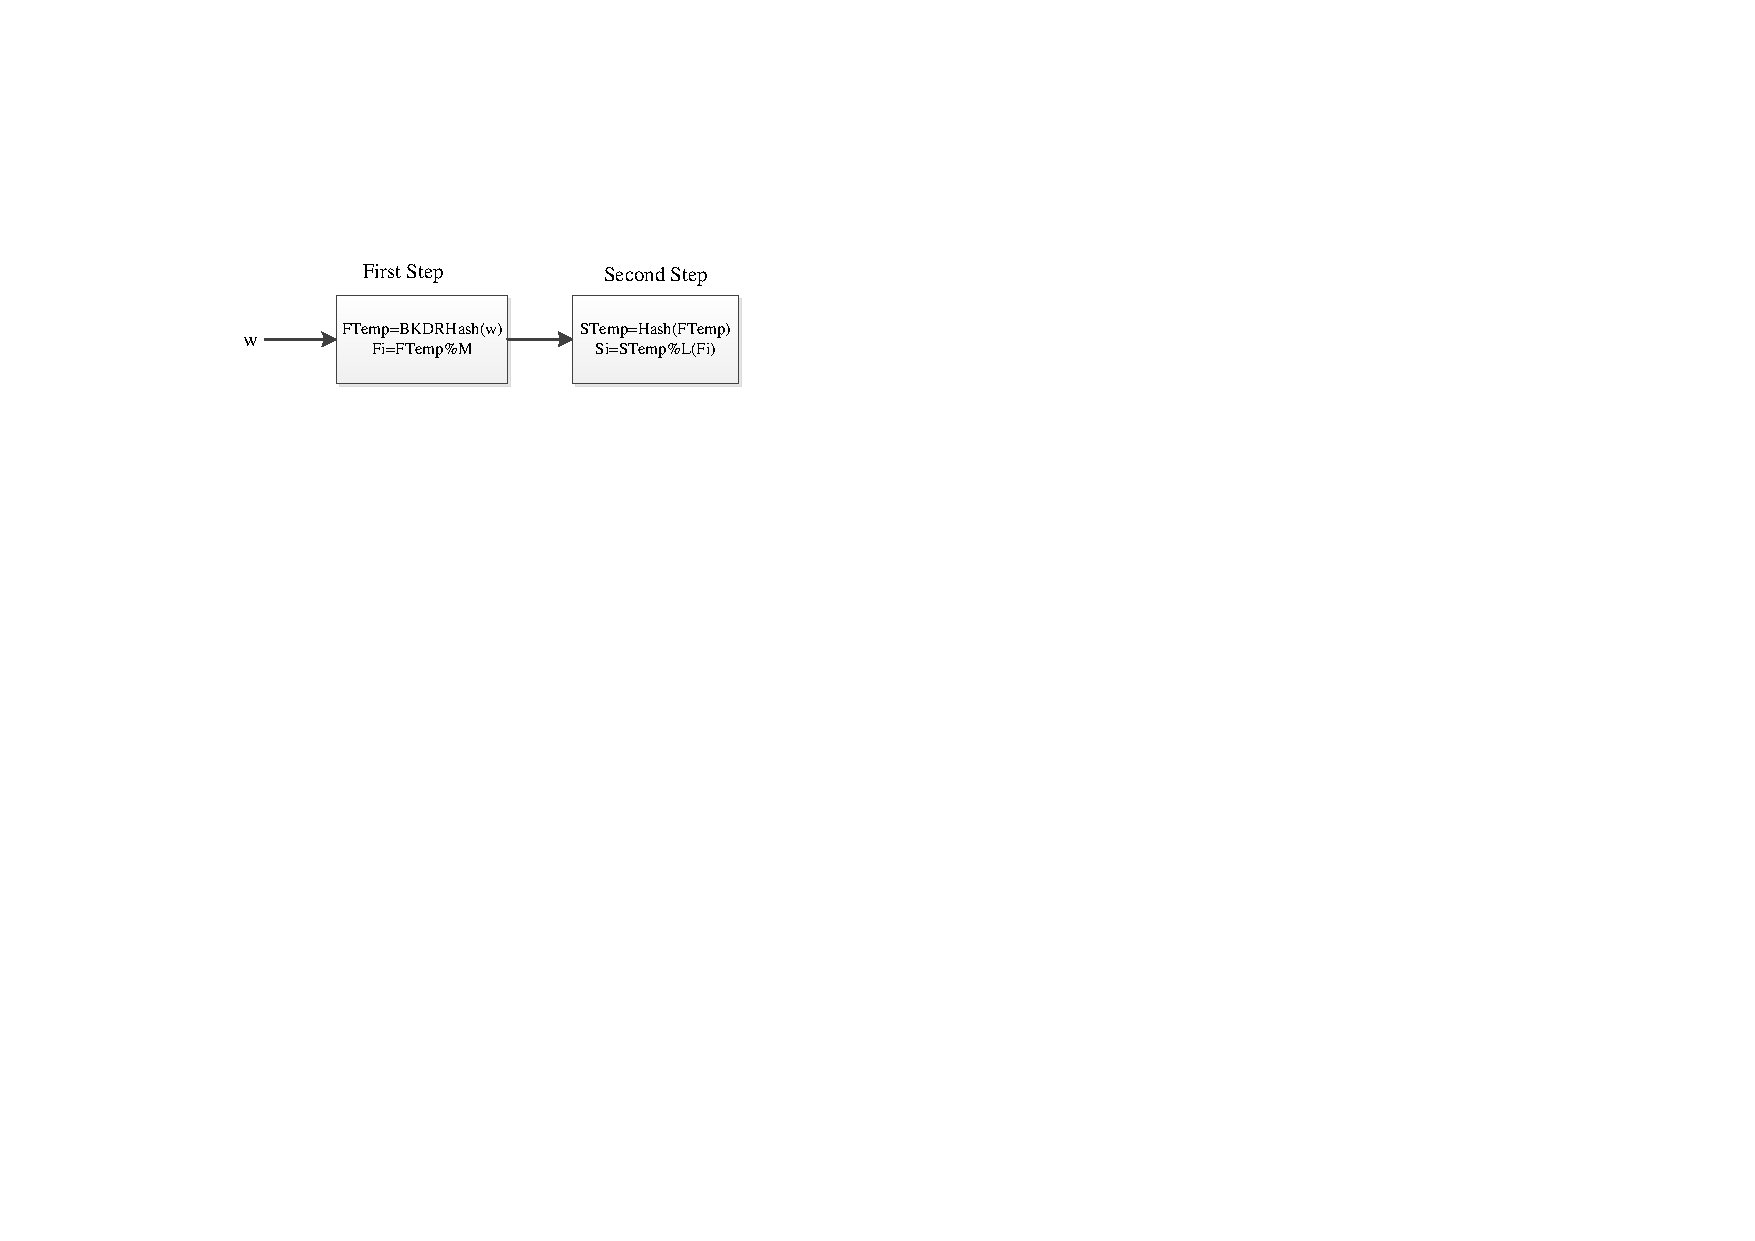
\includegraphics[width=3.5in,height=0.6in]{HASH}
\caption{The Hash Function} \label{F20}
\end{figure}

As illustrated in Fig. \ref{F20}, we determine the index of an entry in two steps. In the first step, we first map the keyword w of entry to the FTemp with the string hash function BKDRHash. It's worth to note that, although we apply BKDRHash as hash function, others string hash function can also be applied. And then, we obtain the $Fi$ by performing a modulus on FTemp with first-level index length M. In the second step, we hash the FTemp with an integer hash function and then perform a modulus on STemp with second-level index length of $Fi$ to get $Si$. After these two steps, each KHT entry has an index $(Fi,Si)$. Note that, a delicate situation arises when two or more entries share the same index $(Fi,Si)$ whose probability less than 0.5, which is demonstrated in \cite{cormen2001introduction}. In this case, \textbf{\textit{``linear probing''}} technique is utilized to tackle this problem. From Table \ref{T4} we know that there is a conflict situation between ``forest'' and ``shore''. As illustrated in Fig. \ref{F1}, when we try to insert the entry $e_4$ into KHT, $e_2$ has already stayed in location $(6,1)$. Due to location $(6,2)$ is occupied as well, with ``linear probing'', $e_4$ is inserted into $(6,3)$ ultimately, just as the solid arrow shown.

With KHT, for a specific query q we can retrieve the $RO_q$ in nearly $\Theta(|q.\omega|)$, and prune the unnecessary visits hugely.








